\documentclass[journal]{IEEEtran}
\usepackage{amsmath,amssymb,booktabs,array,graphicx,cite,xurl,balance}
\usepackage[hidelinks]{hyperref}
\hypersetup{pdftitle={Supplementary Evidence and Reproduction Records: Hierarchical RF Tokenization},pdfauthor={Anonymous working draft}}
\graphicspath{{figures/}}
\begin{document}
\title{Supplementary Evidence and Reproduction Records}
\author{Anonymous working draft}\maketitle
\section{All New Fits and Common Inference}
Only Long-Patch is newly trained. Every fit uses 200 epochs and minimum source RX-equal CE selection. The six source/Dev pairs below are complete, without deleting a weak seed. Target inference occurs after the full source seal. H0/P0 are reused weights; the primary comparison re-evaluates all three arms with identical current GPU precision flags. Historical CPU/GPU values remain separately archived.
\begin{table*}[t]\centering\caption{All six Long-Patch fits; no replacement seeds.}\label{tab:allfits}
\begin{tabular}{rrrrrrr}\toprule
Fold&Seed&Epochs&Best epoch&Source acc.(\%)&Dev acc.(\%)&Fit wall(s)\\\midrule
0&201&200&156&95.250&91.070&2167.7\\
0&202&200&171&96.550&95.330&2162.8\\
0&203&200&171&96.700&95.780&2158.1\\
1&201&200&129&96.100&94.280&2155.4\\
1&202&200&159&96.900&96.120&2123.6\\
1&203&200&153&96.650&94.420&2125.7\\
\bottomrule\end{tabular}\end{table*}
The original S26 registration, data-free resource/recovery gate, source recovery, checkpoint/configuration/history seal, access log, saved predictions, and final recomputation audit provide the evidence chain. Summed per-fit wall times overlap under concurrent jobs and are not active GPU time. Atomic recovery restores optimizer, global and data-stream RNG states at a completed epoch; it does not reset a seed after observing a score.

\section{Kernel, Equivalence, and Metadata Evidence}
\subsection{Kernel Evidence and Its Limits}
Existing S23 effective-kernel spectra are reused. High-frequency energy over 0.25--0.5 cycles per frontend position averages 21.808/7.692/4.043\% for P0/S1/H1. Across the 18-model descriptive join, energy has Spearman correlation $-.556$ with final $J_w$ and $+.410$ with final conditional RX scatter. Arm, cohort, parameterization, and optimization confound the association (Fig.~\ref{fig:kernels}).

\begin{figure*}[t]\centering
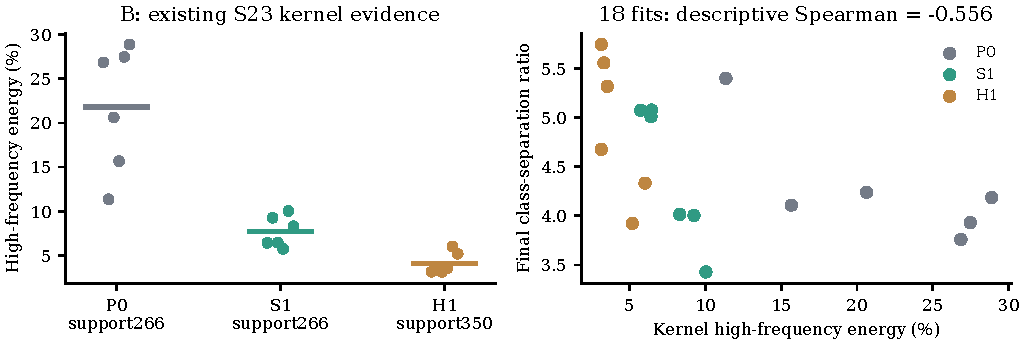
\includegraphics[width=.96\textwidth]{fig04_mechanism_B.pdf}
\caption{Mechanism B. Existing effective-kernel spectra and support (left) joined to new frozen source features (right). These filters act on frontend coordinates, not physical transmitter spectra. All 18 applicable fits are retained.}
\label{fig:kernels}
\end{figure*}

S23 materialized six S1 models as ordinary 256-tap convolutions with bit-identical logits on 12,000 source predictions. For effective kernel $v=Tw$, $T$ has rank 256: the inference function class need not shrink, while optimization coordinates change. A $TT^\top$ interpretation for idealized SGD is not the exact update of AdamW.

Frozen BN can be absorbed into preceding convolutions, but numerical execution matters. Default TF32-enabled execution failed the fixed logit tolerance in all six H0 checks (maximum difference about .01957), although classifications agreed. Disabling TF32 passed the same $10^{-4}$ tolerance (maximum $5.39\times 10^{-5}$). These failures distinguish training effects from removable inference structure.

\subsection{Source Metadata Diagnostics}
Only selected legal source-validation rows of supplied CFO/SNR fields were read. That loader does not read the waveform dataset, the fields never enter a network, and no target CFO/SNR was opened. Raw Spearman correlations with true-class margin are accompanied by fixed TX-by-RX-cell centering; constant residuals are NA.

Across 24 models, raw SNR--margin correlations are negative, but centered correlations range approximately $-.028$ to $.058$. Centered absolute-CFO correlations range approximately $-.057$ to $.032$. This does not establish absence of RF effects: metadata, identity, acquisition, and margin scale are intertwined. It illustrates why raw associations cannot explain held-RX errors. Raw and cosine-weight margins include misclassified samples and every fit.


\section{Complete External RX Attribution}
These are the original S24 external and S22 matched archival GPU cohorts. The heatmap retains the two receivers where H0 loses to Native Shen-DANN and the concentration at Pluto-1. Its H0/P0 archival cohort is explicitly distinct from the new S26 common inference.
\begin{figure*}[t]\centering
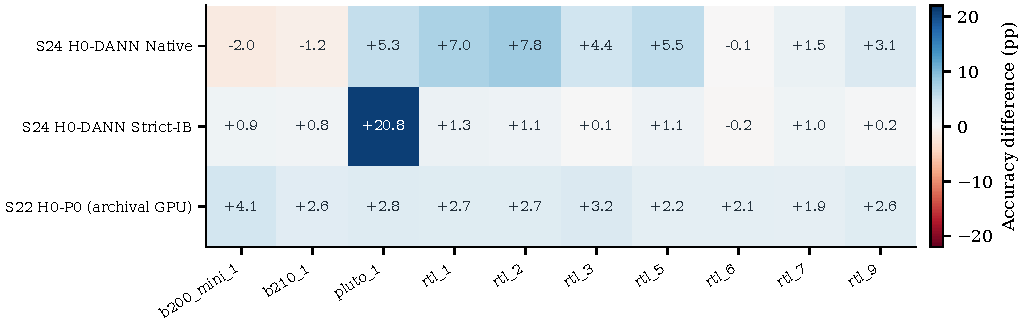
\includegraphics[width=.97\textwidth]{fig05_mechanism_C.pdf}
\caption{Mechanism C: all ten RXs. S24 H0--DANN uses the common new evaluation; H0--P0 is explicitly the matched archival GPU cohort. Positive favors H0. Neither is a newly independent test.}
\label{fig:rx}
\end{figure*}
\section{All Frozen-Source PCA Cohorts}
All four arms and all six fold/seed cohorts are included. Each model uses its own deterministic top-two PCA components of final per-packet L2 features. Colors identify TX31--40; shapes identify source RXs. These are 50 cell centroids, not the full sample cloud; two-dimensional appearance is not quantitative evidence or independent generalization.
\begin{figure*}[t]\centering
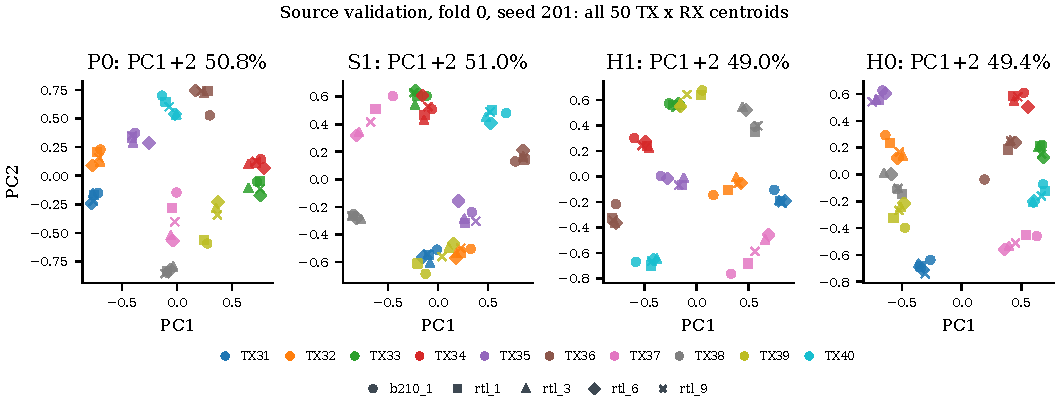
\includegraphics[width=.98\textwidth]{supp_pca_f0_s201.pdf}
\caption{All source TX-by-RX centroids, fold 0, seed 201. Separate model coordinate systems.}
\end{figure*}
\begin{figure*}[t]\centering
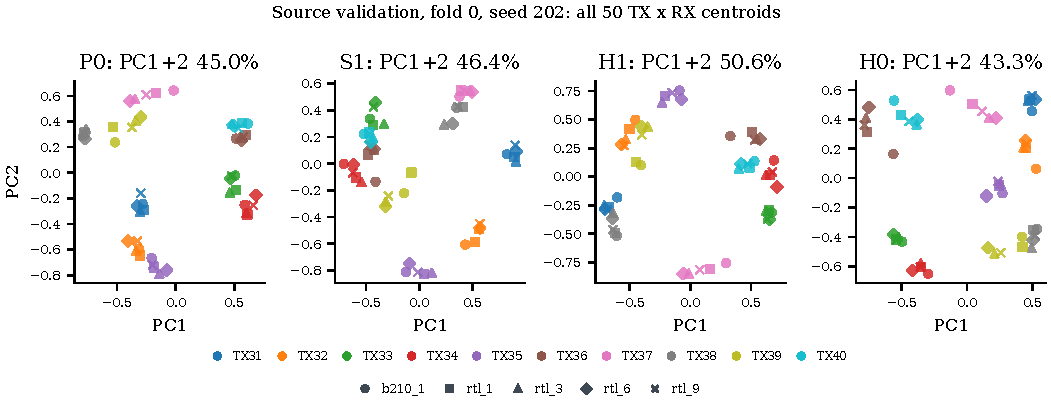
\includegraphics[width=.98\textwidth]{supp_pca_f0_s202.pdf}
\caption{All source TX-by-RX centroids, fold 0, seed 202. Separate model coordinate systems.}
\end{figure*}
\begin{figure*}[t]\centering
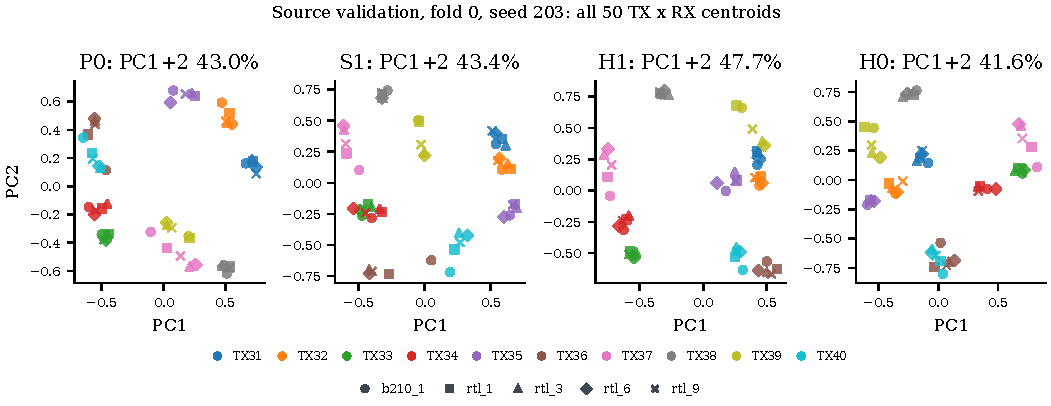
\includegraphics[width=.98\textwidth]{supp_pca_f0_s203.pdf}
\caption{All source TX-by-RX centroids, fold 0, seed 203. Separate model coordinate systems.}
\end{figure*}
\begin{figure*}[t]\centering
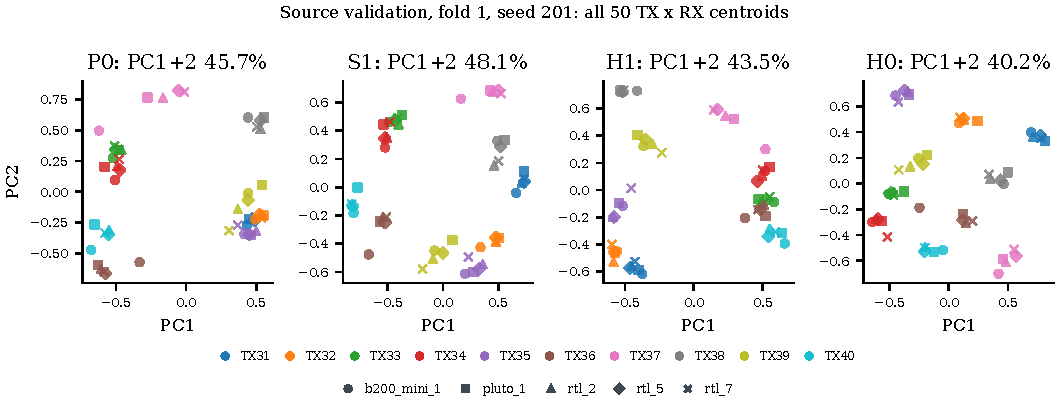
\includegraphics[width=.98\textwidth]{supp_pca_f1_s201.pdf}
\caption{All source TX-by-RX centroids, fold 1, seed 201. Separate model coordinate systems.}
\end{figure*}
\begin{figure*}[t]\centering
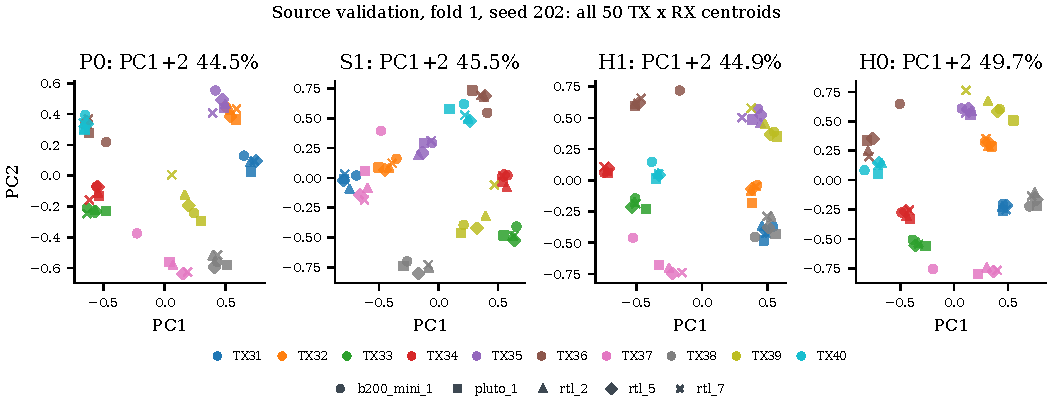
\includegraphics[width=.98\textwidth]{supp_pca_f1_s202.pdf}
\caption{All source TX-by-RX centroids, fold 1, seed 202. Separate model coordinate systems.}
\end{figure*}
\begin{figure*}[t]\centering
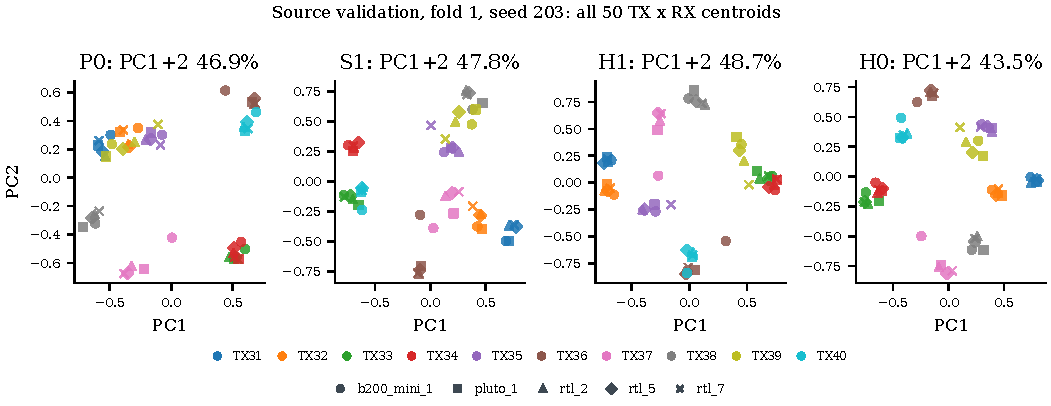
\includegraphics[width=.98\textwidth]{supp_pca_f1_s203.pdf}
\caption{All source TX-by-RX centroids, fold 1, seed 203. Separate model coordinate systems.}
\end{figure*}

\section{Audit Boundaries and Companion Overlap}
The existing source validation packets already selected checkpoints; feature diagnostics are exploratory. TrueIB, five views, local frontend, token geometry, and data origin are inherited from the companion OOB manuscript \cite{oobcompanion}. The old six-RX blind set and Confirm RXs have research history and are not newly independent. No new capture is available. Unknown-TX rejection, FAR/FRR, active spoofing, and calibrated real synchronization-offset robustness are untested.

The S25 TF32-off source analysis retained two net one-packet accuracy changes and one additional changed confusion pattern despite identical weights. Its final ratios are computed from that single analysis execution. S26's separate original-precision source recovery and common target-inference comparisons are recorded without overwriting these historical files. Numeric recovery is an execution observation, not permission to select a better result.

Ma's unpretrained Siamese variant is source-compatible in principle \cite{ma2025robust}; the optional externally pretrained variant requires a separate budget. A checked author implementation and a frozen source-only adapter were not qualified here. No simplified network or paper score substitutes for it. This is a remaining coverage limitation, not proof that the method cannot be adapted.

The ten-claim evidence matrix and ten reviewer answers are updated in the repository. They separate measured system effects, exploratory associations, architectural identities, and unresolved mechanisms. Full negative shift and weak-fit results are retained.
\clearpage
\bibliographystyle{IEEEtran}
\bibliography{references}
\end{document}
